\documentclass[11pt]{standalone}

\usepackage{ifthen}
\usepackage{tikz} 
\usetikzlibrary{shapes.misc}
\usetikzlibrary{arrows,arrows.meta}
\usetikzlibrary{calc,intersections, patterns, math}

\definecolor{pfeil}{RGB}{168,167,167}
\definecolor{petrol}{RGB}{0, 118, 136}
\definecolor{darkgoldenrod}{RGB}{184, 134, 11}
\colorlet{petrol-lighter}{petrol!40}
\colorlet{darkgoldenrod-lighter}{darkgoldenrod!40}

\begin{document}

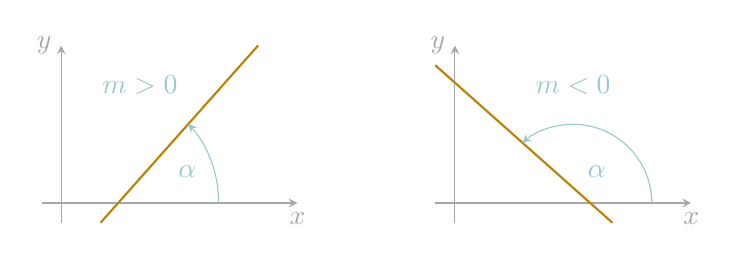
\begin{tikzpicture}[pfeil]

    % \draw[thick, fill=petrol!20, draw=petrol-lighter, rounded corners=2ex, opacity=0.5] (0,0) rectangle ++ (1.5,3.5);
    % \draw[thick, fill=darkgoldenrod!20, draw=darkgoldenrod-lighter, rounded corners=2ex, opacity=0.5] (5,0) rectangle ++ (1.5,3.5);

        \draw[pfeil,-stealth] (-0.25,0) -- (3,0) node[below]{$x$};
        \draw[pfeil,-stealth] (0,-0.25) -- (0,2) node[left]{$y$};
        
        \draw[thick, darkgoldenrod] (0.5,-0.25) -- (2.5,2);
        \draw[petrol-lighter,-stealth] (2,0) arc(0:42:1.5);
        
        \node[petrol-lighter] at (1,1.5) {$m>0$};
        
        \node[petrol-lighter] at (1.6,0.4) {$\alpha$};
        
        \begin{scope}[xshift=5cm]
            \draw[pfeil,-stealth] (-0.25,0) -- (3,0) node[below]{$x$};
            \draw[pfeil,-stealth] (0,-0.25) -- (0,2) node[left]{$y$};
            
            \draw[thick, darkgoldenrod] (-0.25,1.75) -- (2,-0.25);
            \draw[petrol-lighter,-stealth] (2.5,0) arc(0:130:1);
            
            \node[petrol-lighter] at (1.5,1.5) {$m<0$};
            \node[petrol-lighter] at (1.8,0.4) {$\alpha$};
        \end{scope}
    

\end{tikzpicture}

\end{document}
